\documentclass[11pt, oneside]{article} 
\usepackage{geometry}
\geometry{letterpaper} 
\usepackage{graphicx}
	
\usepackage{amssymb}
\usepackage{amsmath}
\usepackage{parskip}
\usepackage{color}
\usepackage{hyperref}

\graphicspath{{/Users/telliott/Github/number_theory/png/}}
% \begin{center} 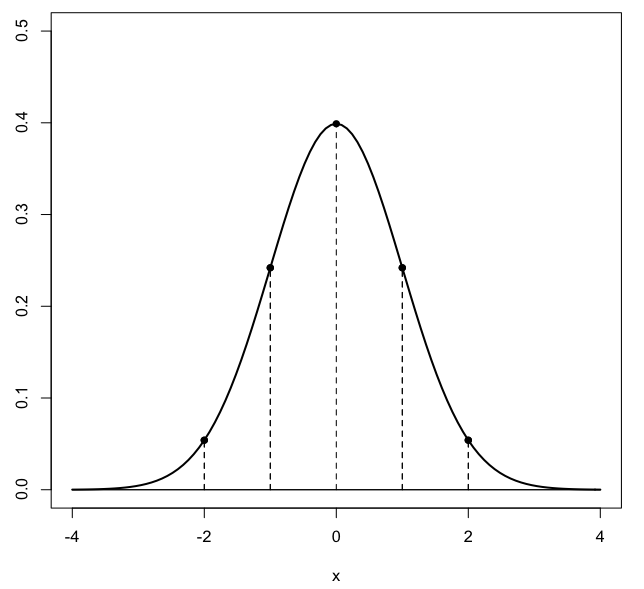
\includegraphics [scale=0.4] {gauss3.png} \end{center}

\title{Hardy proof of FTA}
\date{}

\begin{document}
\maketitle
\Large

We will prove that every integer has a unique \emph{prime factorization}.  

Examples:
\[ 6006 = 2 \cdot 3 \cdot 7 \cdot 11 \cdot 13 \]
\[ 144 = 2 \cdot 2 \cdot 2 \cdot 2 \cdot 3 \cdot 3 \]
\[ 12 = 2 \cdot 2 \cdot 3 \]

This is also called \emph{the fundamental theorem of arithmetic}.

\[ n = p_1 \cdot p_2 \dots p_k \]

In the list of the prime factors of $n$, a factor may be repeated.  To compare two factorizations for uniqueness, we suppose they are sorted (say, from smallest to greatest).

\subsection*{proof}

Hardy and Wright (\emph{Theory of Numbers}, sect. 2:11) have a proof of prime factorization, different than the standard one, which I find quite elegant.

But its great virtue is that it simplifies the proof of Euclid's lemma, which leads to Bezout's identity, and that proof is tedious.

It is a proof by contradiction.

\begin{quote}Let us call numbers which can be factored into primes in more than one way, \emph{abnormal}, and let $n$ be the smallest abnormal number.\end{quote}

\subsection*{Different factorizations}

As a preliminary result, the same prime $P$ cannot appear in two different factorizations of $n$, for, if it did, $n/P$ would be abnormal and yet $n/P < n$, the smallest abnormal number.

Thus, we have that

\[ n = p_1 \cdot p_2 \dots p_k \]
and
\[ n = q_1 \cdot q_2 \dots q_j \]
    
where the $p$ and $q$ are primes, and no $p$ is a $q$ and no $q$ is a $p$.

If there do exist abnormal numbers with two factorizations, those factorizations must be completely different.

\subsection*{setup}

In this part, we establish that $p_1 \cdot q_1 < n$.

We may take $p_1$ to be the least $p$ and $q_1$ to be the least $q$.  

Since $n$ is composite, either $p_1^2 = n$ (and $p_1$ is the only factor of $n$),

Or $p_1$ times the largest $p_k = n$, so $p_1 < p_k$, $p_1 p_k = n$ and so $p_1^2 < n$.

A similar result holds for $q_1$, but since $p_1 \ne q_1$, either $p_1^2 < n$ or $q_1^2 < n$ or perhaps both statements are true.

From this, it follows that $p_1 q_1 < n$. 

\subsection*{the contradiction} 

Let $N = n - p_1 q_1$.

We have $0 < N < n$ and also that $N$ is not abnormal.

We're given that $p_1 | n$ and so, from the above equality, it must be that $p_1 | N$.

A similar result is true for $q_1$, namely $q_1 | N$.  

Hence both $p_1$ and $q_1$ appear in the unique factorizations of both $N$ and $p_1 q_1$.

From this it follows that $p_1 q_1 | n$ and hence $q_1 = n/p_1$.  

But $n/p_1$ is less than $n$ and has the unique prime factorization $p_2 p_3 \dots p_k$.

Since $q_1$ is not a $p$, this is impossible.  

Hence there cannot be any abnormal numbers, and this is the fundamental theorem.

$\square$

\end{document}